\documentclass[12pt]{article}
\usepackage[table]{xcolor}
\usepackage[shortlabels]{enumitem}
\usepackage{tabularx,xltabular}
\usepackage{graphicx}
\usepackage{hyperref}
\usepackage{verbatim}
\usepackage{geometry}
\usepackage{ulem}
\usepackage[official]{eurosym}
\usepackage{tikz}
\usetikzlibrary{arrows,backgrounds,calc,decorations.markings,patterns,3d}
\usepackage{pgfplots}
\pgfplotsset{compat = newest}
\usetikzlibrary{fit}
\newcommand\addvmargin[1]{
\usetikzlibrary{arrows}
\node[fit=(current bounding box),inner ysep=#1,inner xsep=0]{};}
\usepackage{cancel}
\usepackage{fontspec}
\usepackage{array}  
\geometry{a4paper, top=2cm, left=2cm, right=2cm, bottom=2cm, headsep=1cm}
\usepackage{tabu}
\usepackage{pst-node}
\usepackage{colortbl}
\usepackage{array}
\usepackage{german}
\setlength\parindent{0pt}
\newcolumntype{?}{!{\vrule width 1pt}}
\usepackage{makecell}
\renewcommand{\arraystretch}{2.5}
\usepackage{pbox}
\usepackage{amssymb}
\usepackage{amsmath}
\usepackage{booktabs}
\newcolumntype{L}[1]{>{\raggedright\let\newline\\\arraybackslash\hspace{0pt}}m{#1}}
\newcolumntype{C}[1]{>{\centering\let\newline\\\arraybackslash\hspace{0pt}}m{#1}}
\newcolumntype{R}[1]{>{\raggedleft\let\newline\\\arraybackslash\hspace{0pt}}m{#1}}
\begin{document}
\rightline{Datum: 08.06.2023}
\centerline{{\Large Tägliche Übungen}} 
\vspace{1cm}
\noindent \\


\begin{xltabular}{\textwidth}{|C{0.75cm}|X|C{0.75cm}|X|}
\arrayrulecolor{black}\hline
a)&$10\cdot x + 6\cdot x=12 + 8$
&
b)&$2\cdot x - 10=3 + 9\cdot x$
\\\hline
c)&$12 + 10=11\cdot x + 11$
&
\end{xltabular}
\vspace{0.5cm}
\newpage
\rightline{Datum: 08.06.2023}
\centerline{{\large Lösungen Tägliche Übungen}} 
\vspace{0.5cm}

\begin{xltabular}{\textwidth}{|C{0.75cm}|X|C{0.75cm}|X|}
\arrayrulecolor{black}\hline
a)&\begingroup\setlength{\jot}{-0.03cm}
\tikzstyle{background grid}=[draw, black!15,step=.5cm]
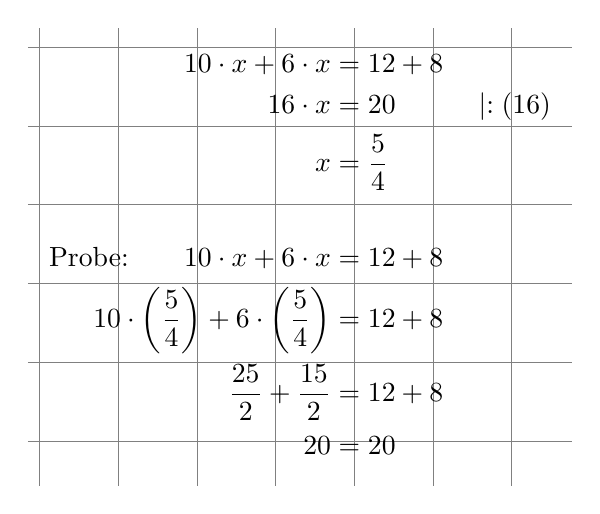
\begin{tikzpicture}[show background grid]
\node[below right] at (0,0.1) {
$\begin{aligned}
10\cdot x + 6\cdot x &=12 + 8& &  \\
16\cdot x &=20& & \mid :\left(16\right)\\
x &={{\frac{5}{4}}}& & 
\\
\\
\mbox{Probe:}\qquad 10\cdot x + 6\cdot x &=12 + 8& &  \\
10\cdot \left({{\frac{5}{4}}}\right) + 6\cdot \left({{\frac{5}{4}}}\right) &=12 + 8& &  \\
{{\frac{25}{2}}}+{{\frac{15}{2}}} &=12+8& &  \\
20 &=20& &  \\
\end{aligned}$};
\end{tikzpicture}
\endgroup
&
b)&\begingroup\setlength{\jot}{-0.03cm}
\tikzstyle{background grid}=[draw, black!15,step=.5cm]
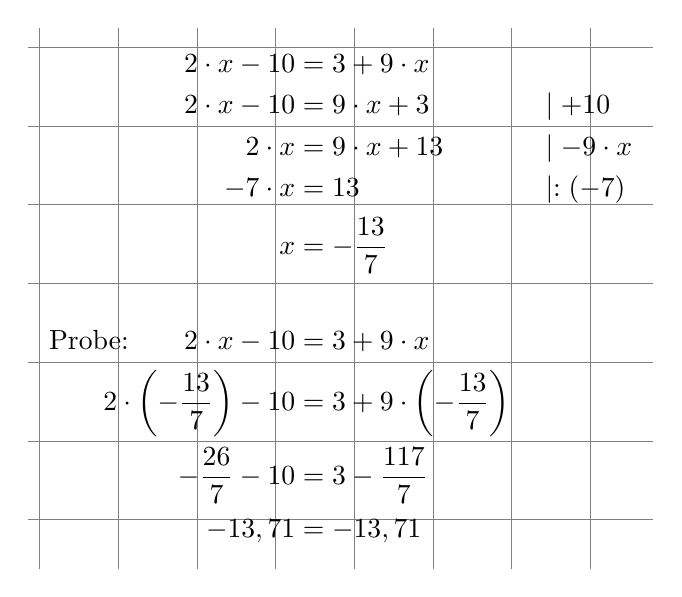
\begin{tikzpicture}[show background grid]
\node[below right] at (0,0.1) {
$\begin{aligned}
2\cdot x - 10 &=3 + 9\cdot x& &  \\
2\cdot x - 10 &=9\cdot x + 3& & \mid + 10\\
2\cdot x &=9\cdot x + 13& & \mid -9\cdot x \\
-7\cdot x &=13& & \mid :\left(-7\right)\\
x &=-{{\frac{13}{7}}}& & 
\\
\\
\mbox{Probe:}\qquad 2\cdot x - 10 &=3 + 9\cdot x& &  \\
2\cdot \left(-{{\frac{13}{7}}}\right) - 10 &=3 + 9\cdot \left(-{{\frac{13}{7}}}\right)& &  \\
-{{\frac{26}{7}}}-10 &=3-{{\frac{117}{7}}}& &  \\
-13,71 &=-13,71& &  \\
\end{aligned}$};
\end{tikzpicture}
\endgroup
\\\hline
c)&\begingroup\setlength{\jot}{-0.03cm}
\tikzstyle{background grid}=[draw, black!15,step=.5cm]
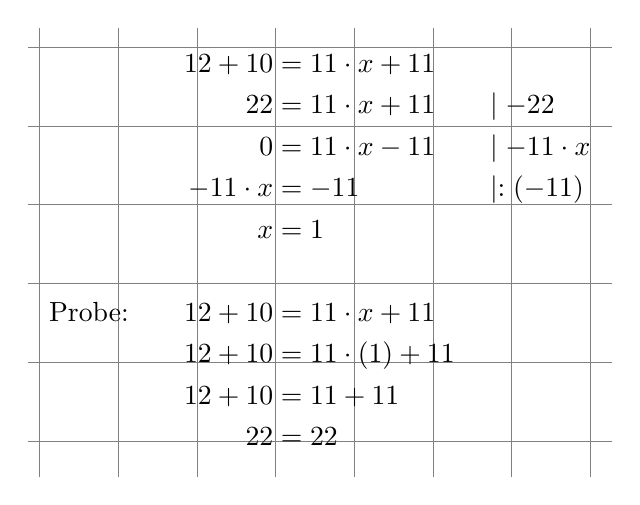
\begin{tikzpicture}[show background grid]
\node[below right] at (0,0.1) {
$\begin{aligned}
12 + 10 &=11\cdot x + 11& &  \\
22 &=11\cdot x + 11& & \mid -22\\
0 &=11\cdot x - 11& & \mid -11\cdot x \\
-11\cdot x &=-11& & \mid :\left(-11\right)\\
x &=1& & 
\\
\\
\mbox{Probe:}\qquad 12 + 10 &=11\cdot x + 11& &  \\
12 + 10 &=11\cdot \left(1\right) + 11& &  \\
12+10 &=11+11& &  \\
22 &=22& &  \\
\end{aligned}$};
\end{tikzpicture}
\endgroup
&
\end{xltabular}
\vspace{0.5cm}
\end{document}